\documentclass{article}
\usepackage[utf8]{inputenc}
\usepackage[T1]{fontenc}
\usepackage[ngerman]{babel}
\usepackage{microtype}
\usepackage{graphicx}
\usepackage{float}
\usepackage{subcaption}
\usepackage{hyphenat}
\usepackage{natbib}
\usepackage{url}
\usepackage{amsmath}
\usepackage{booktabs}

%%%%%%%%%%%%%%%%%%%%%%%%%%%%%%

\begin{document}

\title{KI-basierte IGRT mit 2D-bildgeführtem Dose Tracking täglicher
Conebeam-CTs zur Bewertung der Prostatalage, Füllung von Rektum und Harnblase
bei definitiver Radiotherapie des Prostatakarzinoms}
% \author{Peter Rhone, Dipl. Phys., Prof. Dr. med. Thomas Kuhnt, Dr. med. Franziska Nägler}
\author{\begin{minipage}{0.8\textwidth}\centering \small Peter Rhone,
Dipl.-Phys., Prof. Dr. med. Thomas Kuhnt, \\ Dr. med. Franziska
Nägler\end{minipage}} \maketitle

% \tableofcontents
\vspace{2cm}

\begin{abstract}
Es wird eine Methode zur automatischen Erkennung von Harnblase und Rektum in
täglichen Cone-Beam-CTs (kV-CBCTs) für die bildgesteuerte Strahlentherapie
(IGRT) vorgestellt. Mediale sagittale Schnitte – zentral durch die Symphyse
sowie links und rechts davon – wurden mittels künstlicher Intelligenz (KI)
segmentiert, um die Organlage sowie die Füllungszustände von Rektum und
Harnblase bei der definitiven Radiotherapie des Prostatakarzinoms zu bewerten.
Das Modell wurde mit Daten von 131 Patienten trainiert und validiert (jeweils 5
CBCTs pro Patient). Die Ergebnisse zeigen eine hohe Segmentierungsgenauigkeit
mit Dice-Koeffizienten von etwa 0,98 für Harnblase und Prostata-PTV sowie 0,95
für das Rektum.
\end{abstract}

\section{Einleitung}
% INTRODUCTION  
% Sets the stage by providing background information on the topic.  
% Identifies the problem or gap in knowledge that the research addresses 
% (e.g., a challenge in healthcare data management or clinical decision support).  
% States the study’s objectives or research questions and its significance in the 
% context of medical informatics.
Bei der definitiven Bestrahlung von Prostatakarzinomen niedrigen und mittleren
Risikos werden in unserer Einrichtung kurative Dosen von 68~Gy in moderater
Hypofraktionierung appliziert \citep{ethik2024}. Intrafraktionelle Variabilität,
wie Füllungszustände oder Organbewegungen, kann dazu führen, dass Risikoorgane
wie Harnblase und Rektum unerwünscht hohe Dosen erhalten, was die akute oder
chronische Toxizität erhöhen kann \citep{kupelian2007, quantec}. Die
bildgesteuerte Strahlentherapie (IGRT) mit Cone-Beam-CTs (CBCTs) verifiziert die
Organlagen vor jeder Fraktion. Jedoch erschweren variierende Füllungen – etwa
eine schlecht gefüllte Harnblase oder ein luftgefülltes Rektum – das Einhalten
von Dosis-Constraints wie \( V_{65} < 50\,\% \) für die Harnblase
\citep{wang2022, quantec}. Online-adaptive Strahlentherapie ermöglicht eine
tägliche Anpassung an diese Veränderungen, erfordert jedoch erheblichen
Personalaufwand (15–35 Minuten pro Fraktion) \citep{byrne2022}, was in
Hochdurchsatz-Kliniken kaum umsetzbar ist. Häufig wird nur ein Offline-Review
durchgeführt, bei dem Abweichungen erst nachträglich erkannt werden. Diese
Studie entwickelt eine KI-basierte Methode zur teilweisen Automatisierung der
online-adaptiven Therapie, inspiriert von Fortschritten in der medizinischen
Bildsegmentierung \citep{litjens2017}, um die Prostatalage und Organfüllung
effizienter zu überwachen und die Behandlungsqualität zu verbessern.


\section{Methoden}
% METHODS  
% Describes how the research was conducted so others can replicate or evaluate
% it.  Includes details like study design (e.g., observational, experimental,
% or system development), data sources (e.g., electronic health records,
% surveys), tools/technologies used (e.g., machine learning algorithms,
% databases), and analysis methods.  May also cover ethical considerations,
% such as patient data privacy or institutional review board approval.
Zwischen dem 01.07.2019 und dem 31.01.2024 wurden retrospektiv 131 Patienten mit
Prostatakarzinom niedrigen bis mittleren Risikos ausgewählt, die eine
definitive, moderat hypofraktionierte Radiotherapie (25 Fraktionen, 58–68\,Gy)
erhielten \citep{ethik2024}. Einschlusskriterien waren cT1a–cT2b, PSA \(\leq
20\,\text{ng/ml}\) und Gleason-Score \(\leq 7\); Patienten mit Hochrisikoprofil
oder Fernmetastasen wurden ausgeschlossen. Eine schriftliche Einwilligung zur
anonymen Datenverwendung liegt vor.

Für jeden Patienten wurden ein Planungs-CT (PL-CT) und 5 kV-CBCTs aus dem
RayStation-System (Versionen 10B–12A) anonymisiert extrahiert \citep{zwart2022}.
Strukturen (Prostata-PTV, Harnblase, Rektum u.a.) wurden manuell von einem
Medizinphysiker konturiert und von einem Facharzt überprüft. Ein selbst
entickeltes Python-Programm (\textit{sqlite\_dicom2.py}) \cite{rhone_repo} konvertierte
DICOM-Daten in Volumina, extrahierte drei mediale sagittale 2D-Schnitte pro CBCT
– eine zentrale Schicht durch die Symphyse sowie je eine links und rechts davon
– und generierte Binärmasken der Konturen mittels der \textit{ConvexHull}
Funktion aus dem \textit{SciPy}-Bibliothek. Die Ausgaben (Patientennummer,
DICOM-Serie, Schnittbilder, Maske, Schnittnummer) wurden in eine
SQLite-Datenbank gespeichert. Ein zweites Sonderprogramm
(\textit{sqlite\_viewer.py}) \cite{rhone_repo} ermöglichte die visuelle
Überprüfung und Datenbereinigung.

Die Bilder wurden präprozessiert (Entfernung von Bildern ungewöhnlicher Größen,
Normalisierung der Pixeldaten). Insgesamt entstanden pro Organ ca. 2100 Bilder
(3 Schnitte × 5 CBCTs × 131 Patienten), wovon etwa 1700 für das Training und
etwa 400 für die Validierung genutzt wurden.  Patienten dessen Bilder für das
Training genutzt wurden, wurden aus dem Validierungsdatensatz ausgeschlossen.
Zur Qualitätssteigerung wurden die 1700 Trainingsbilder durch Augmentation
vervielfältigt – zufällige Rotation, Spiegelung, Zerrung, und Rauschen –
wodurch etwa 9000 Bilder generiert wurden, eine bewährte Methode zur
Verbesserung der Modellrobustheit in der Bildsegmentierung
\citep{ronneberger2015, pereira2016, shorten2019}.

Ein Convolutional Neural Network (CNN) basierend auf U-Net
\citep{ronneberger2015} wurde mit PyTorch trainiert, beschleunigt durch den
ROCm-Stack auf einer AMD RX 7900 XTX GPU mit 24 GB VRAM. Das Modell besteht aus
einer Encoder-Decoder-Architektur mit Faltungsblöcken (jeweils zwei \(3 \times
3\)-Faltungen mit ReLU-Aktivierung) und transponierten Faltungen für die
Upsampling-Schichten. Es wurde mit einer Lernrate von \(10^{-4}\) und dem
Adam-Optimierer über 25 Epochen trainiert, wobei die binäre Kreuzentropie mit
Logits (\textit{BCEWithLogitsLoss}) als Verlustfunktion diente. Nur CBCT-Daten
wurden zum Training verwendet, um Konsistenz zu gewährleisten
\citep{litjens2017}. Die Trainingsdaten wurden in einem benutzerdefinierten
\textit{ImageDataset} als PyTorch-Tensoren (aus Pandas-Series gestapelt)
organisiert und mit einem \textit{DataLoader} (Batch-Größe 32, 4 Worker,
\textit{pin\_memory=True}) geladen. Während des Trainings wurden Bilder und
Masken batchweise auf die GPU verschoben, der Verlust nach jedem Batch
rückpropagiert und optimiert. Die Trainingszeit betrug ca. 1 Stunde pro Organ.

Das Blasenvolumen wurde grob geschätzt, indem Höhe und Breite der Blasenmaske in
der mittleren sagittalen Ebene gemessen und das Volumen eines prolaten Sphäroids
berechnet wurden. Für das Rektum wurde das Volumen eines Zylinders zur Schätzung
herangezogen.


\section{Ergebnisse}
% RESULTS  
% Presents the findings of the study without interpretation.  
% Uses text, tables, charts, or figures to display data clearly 
% (e.g., system performance metrics, statistical outcomes, or user adoption rates).  
% Organized logically, often aligning with the methods section.
Das U-Net-Modell wurde pro Organ auf etwa 400 Validierungsbilder getestet. Die
Segmentierungsgenauigkeit zeigte folgende Dice-Koeffizienten, gemittelt über
alle Validierungsbilder:


\begin{table}[H]
  \centering
  \begin{tabular}{lcc} % Left-aligned organ names, centered coefficients and deviations
    \toprule
        Organ & Dice-Koeffizienten & Standardabweichung \\
    \midrule
        Harnblase       & $0.9815$ & $\pm 0.0126$ \\
        Prostata PTV    & $0.9789$ & $\pm 0.0092$ \\
        Rektum          & $0.9552$ & $\pm 0.1021$ \\
    \bottomrule
  \end{tabular}
  \caption{Dice-Koeffizienten und Standardabweichungen für verschiedene Organe.}
  \label{tab:dice_coefficients}
\end{table}

Die Volumina von Harnblase und Rektum wurden geschätzt. Diese Werte können mit
den Volumina aus dem PL-CT verglichen werden, um die Füllungszustände zu
bewerten.

Als „Ground Truth“ dienten die manuell erstellten Konturen, die von einem
Facharzt überprüft wurden. Die Modellvorhersagen wurden visuell mit den
Ground-Truth-Daten verglichen. Beispiele sind in den Abbildungen
\ref{fig:bladder_combined}, \ref{fig:prostate_combined} und
\ref{fig:rectum_combined} dargestellt.
% Bladder Figures
\begin{figure}[H]
    \centering
    \begin{subfigure}[t]{0.9\textwidth}
        \centering
        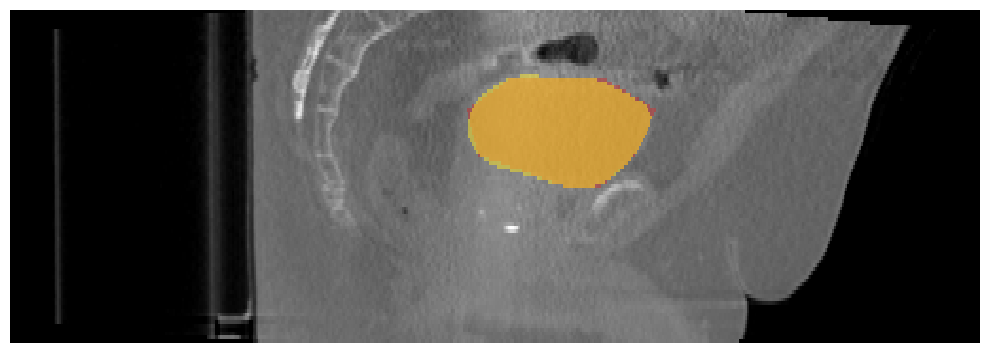
\includegraphics[width=\textwidth]{images/bladder_merged.png}
        \caption{Beispielhafte Segmentierung von Harnblase. Rot: Ground
        Truth, Gelb: Vorhersage, Orange: Übereinstimmung.} \label{fig:harnblasen_segmentation_merged}
    \end{subfigure}
    % \vspace{1cm} % Adjustable vertical space
    \begin{subfigure}[t]{0.9\textwidth}
        \centering
        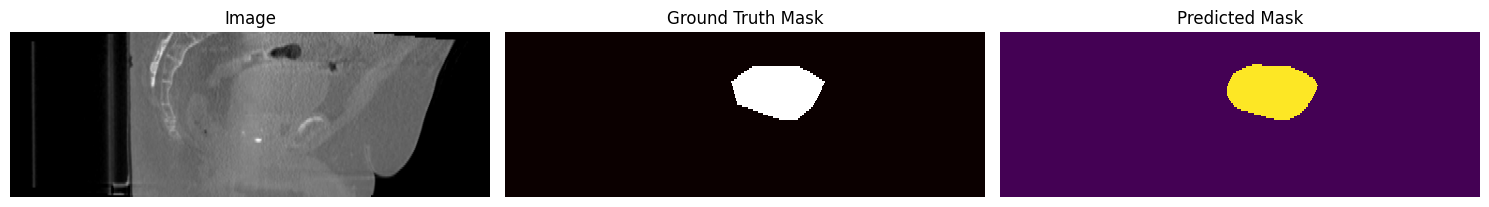
\includegraphics[width=\textwidth]{images/bladder_3_panel.png}
        \caption{Beispielhafte Segmentierung von Harnblase. Links: Originalbild,
        Mitte: Ground Truth, Rechts: Vorhersage des Modells.}
        \label{fig:harnblasen_segmentation}
    \end{subfigure}
    \caption{Gesamtübersicht der Segmentierungsergebnisse für die Harnblase.}
    \label{fig:bladder_combined}
\end{figure}
In Abbildung \ref{fig:harnblasen_segmentation} deckt die Segmentierung die
Harnblase augenscheinlich besser ab als die Ground Truth, die teilweise durch
Segmentierungsartefakte kantig wirkt. Die Modellvorhersage ist glatter und
umfasst die Harnblase vollständig. Die Blasenfüllung wurde in diesem Beispiel
mit 150\,ml geschätzt.
% Prostate Figures
\begin{figure}[H]
    \centering
    \begin{subfigure}[t]{0.9\textwidth}
        \centering
        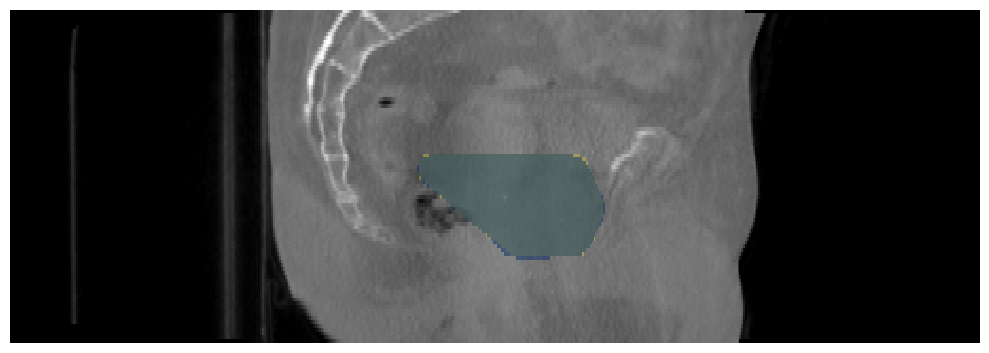
\includegraphics[width=\textwidth]{images/prostate_merged.png}
        \caption{Beispielhafte Segmentierung von Prostata PTV. Gelb: Ground
        Truth, Dunkelblau: Vorhersage, Blaugrün: Übereinstimmung.} \label{fig:prostata_segmentation_merged}
    \end{subfigure}
    % \vspace{1cm}
    \begin{subfigure}[t]{0.9\textwidth}
        \centering
        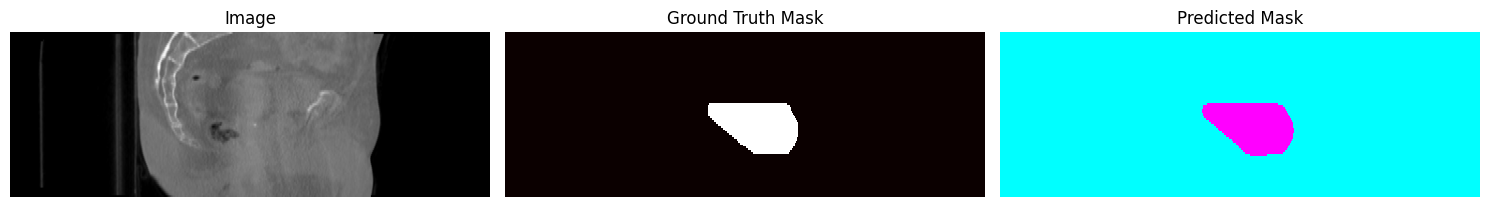
\includegraphics[width=\textwidth]{images/prostate_3_panel.png}
        \caption{Beispielhafte Segmentierung von Prostata PTV. Links:
        Originalbild, Mitte: Ground Truth, Rechts: Vorhersage des Modells.}
        \label{fig:prostata_segmentation}
    \end{subfigure}
    \caption{Gesamtübersicht der Segmentierungsergebnisse für die Prostata PTV.}
    \label{fig:prostate_combined}
\end{figure}
Die Modellvorhersage in Abbildung \ref{fig:prostata_segmentation} deckt die
Prostata-PTV sehr gut ab. Dies ist von fakultativem Interesse, da die PTV keine
klar definierten anatomischen Grenzen wie die Harnblase aufweist. Dennoch kann
die tatsächliche PTV auf das CBCT eingeblendet werden, um die Dosierung an die
Risikoorgane abzuschätzen.
% Rectum Figures
\begin{figure}[H]
    \centering
    \begin{subfigure}[t]{0.9\textwidth}
        \centering
        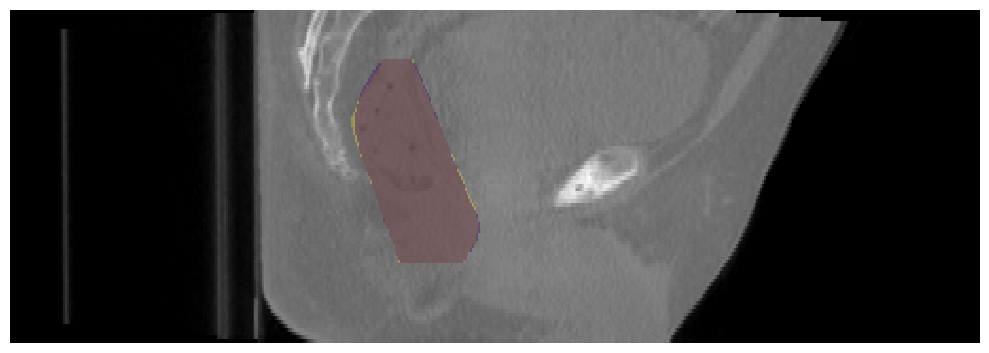
\includegraphics[width=\textwidth]{images/rectum_merged.png}
        \caption{Beispielhafte Segmentierung von Rektum. Gelb: Ground Truth,
        Dunkelbraun: Vorhersage, Hellbraun: Übereinstimmung.}
        \label{fig:rektum_segmentation_merged} \end{subfigure}
    % \vspace{1cm}
    \begin{subfigure}[t]{0.9\textwidth}
        \centering
        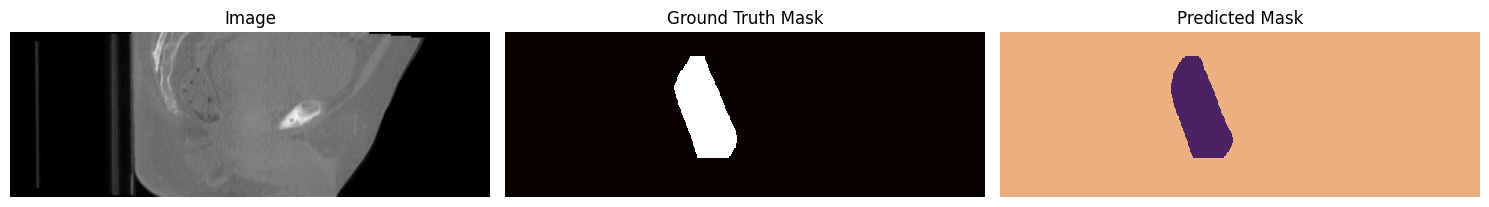
\includegraphics[width=\textwidth]{images/rectum_3_panel.png}
        \caption{Beispielhafte Segmentierung von Rektum. Links: Originalbild, 
        Mitte: Ground Truth, Rechts: Vorhersage des Modells.}
        \label{fig:rektum_segmentation}
    \end{subfigure}
    \caption{Gesamtübersicht der Segmentierungsergebnisse für das Rektum.}
    \label{fig:rectum_combined}
\end{figure}
Die Ergebnisse für das Rektum in Abbildung \ref{fig:rektum_segmentation} sind
ebenfalls zufriedenstellend, jedoch weniger präzise als bei Harnblase und
Prostata-PTV. Dies zeigt sich auch im niedrigeren Dice-Koeffizienten und der
höheren Standardabweichung. Die Rektumfüllung wurde in diesem Beispiel mit
300\,ml geschätzt.
\section{Diskussion}
% DISCUSSION  
% Interprets the results, explaining their meaning and implications.  Compares
% findings with prior research, highlighting similarities, differences, or
% advancements.  Addresses limitations (e.g., sample size, data quality) and
% suggests future research directions.

Die Methode ermöglicht eine präzise Segmentierung von Harnblase und Rektum. Der
Dice-Koeffizient von ~0,98 für Harnblase und Prostata-PTV liefert verlässliche
Ergebnisse für den täglichen Einsatz. Der Wert von ~0,95 für das Rektum ist
ebenfalls akzeptabel, insbesondere in Verbindung mit der Visualisierung. Die
höhere Standardabweichung von ~0,1 für das Rektum spiegelt dessen größere
Variabilität wider \citep{litjens2017}. Die trainierten Modelle können auf einem
handelsüblichen Computer in wenigen Sekunden (nahezu in Echtzeit) ausgeführt
werden, was eine Integration in den klinischen Alltag, etwa als Plugin für das
RayStation-System, ermöglicht.

Eine Erweiterung des Modells auf das gesamte kV-CBCT-Volumen würde eine
3D-Segmentierung der Risikoorgane ermöglichen und die Genauigkeit sowie
Robustheit der Methode steigern. Besonders nützlich wäre die direkte Messung der
Organvolumina. Dies würde jedoch vermutlich eine größere Datenbasis und mehr
Rechenleistung erfordern.

Einschränkungen der Methode umfassen die Abhängigkeit von konsistenten
CBCT-Para\-metern sowie die Ungenauigkeit durch den Informationsverlust bei der
Dimensionsreduktion auf 2D.

Zukünftige Arbeiten könnten Transfer-Learning oder erweiterte Augmentation
einsetzen, um die Robustheit gegenüber variablen Geräten zu verbessern.

\section{Schlussfolgerung}
% CONCLUSION  
% Summarizes the key takeaways and the study’s contribution to medical
% informatics.  May restate the significance or practical applications 
% (e.g., improving patient outcomes or streamlining workflows).
Die KI-basierte Methode automatisiert die Überprüfung von Prostatalage und
Organfüllung effektiv und bietet Potenzial zur Verbesserung der
Behandlungsqualität und Effizienz in der IGRT. Die hohen Dice-Koeffizienten
untermauern die Möglichkeit eines Einsatzes ohne Fiducials (z.\,B. Goldmarker)
in der Prostata, wie derzeit üblich. Sie bildet die Grundlage für breitere
klinische Anwendungen nach weiterer Validierung.

\section{Danksagung}
%ACKNOWLEDGMENTS 
Wir danken der Klinik für Strahlentherapie am Universitätsklinikum Leipzig für
die Datenbereitstellung und technische Unterstützung sowie Prof. Dr. med. Thomas
Kuhnt und Dr. med. Franziska Nägler für die fachliche Betreuung und Saskia
Spautz für die Aufbereitung der Patientendaten.

\section{Literaturverzeichnis}
%REFERENCES  
% Lists all sources cited in the paper, following a specific citation style
% (e.g., APA, AMA, or journal-specific guidelines).  Includes peer-reviewed
% articles, books, or credible technical documentation.
\bibliographystyle{plainnat} 
\bibliography{references} 

\end{document}
